\part{Nivel de Transporte}
\section{Protocolos End-to-End}
Los procesos del nivel de aplicación que usan los servicios de la capa de transporte esperan que proporcione ciertos requisitos:
\begin{itemize}
  \item Garantizar la entrega de mensajes
  \item Entregar mensajes en el mismo orden en que se envían
  \item Entregar a lo sumo una copia de cada mensaje
  \item Soportar mensajes arbitrariamente grandes
  \item Soportar sincronización entre el emisor y el receptor
  \item Permitir al receptor aplicar control de flujo al emisor
  \item Soportar múltiples procesos de aplicación en cada host  
\end{itemize}
\subsection{UDP}
El protocolo de transporte más simple posible es uno que extiende el servicio de entrega de host a host de la red subyacente en un servicio de comunicación de proceso a proceso. Es probable que haya muchos procesos en ejecución en cualquier host dado, por lo que el protocolo necesita agregar un nivel de demultiplexión, lo que permite que varios procesos de aplicación en cada host compartan la red. Aparte de este requisito, el protocolo de transporte no agrega ninguna otra funcionalidad al servicio de mejor esfuerzo proporcionado por la red subyacente. El \textbf{Protocolo de Datagramas de Usuario} (User Datagrama Procol - UDP) de Internet es un ejemplo de este tipo de protocolo de transporte.

Los procesos se identifican indirectamente entre sí utilizando un localizador abstracto, generalmente llamado puerto (\textbf{port}).

La cabecera de un protocolo de extremo a extremo que implementa esta función de demultiplexación típicamente contiene un identificador (puerto) tanto para el remitente (origen) como para el receptor (destino) del mensaje. Es decir, un proceso es realmente identificado por un puerto en algún host en particular, un par \(\langle host, puerto\rangle\).

\subsubsection{Comunicación entre procesos}
\begin{figure}[H]
	\centering
	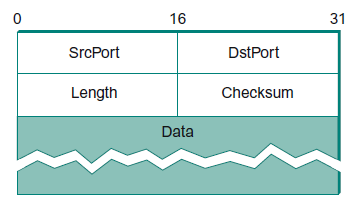
\includegraphics[width=0.5\textwidth
]{images/udp-header.png}
	\caption[Formate de Header para UDP]{Formate de Header para UDP}
	\label{fig:udp-header}
\end{figure}
Típicamente, un proceso cliente inicia un intercambio de mensajes con un proceso servidor. Una vez que el mensaje inicial esrecibido, el servidor conoce el puerto del cliente (del campo \textbf{SrcPrt} contenido en la cabecera del mensaje) y puede responderle. 

Los servidores, esperan recibir mensajes en puertos bien conocidos (\textbf{well-known ports}). Algunos ejemplos:
\begin{itemize}
  \item Los servidores de nombres de dominio (DNS) recibe mensajes en el puerto 53.
  \item El servicio de correo escucha mensajes en el puerto 25.
  \item Unix acepta mensajes en el puerto 517
\end{itemize}

Este mapeo se publica periódicamente en un RFC y está disponible en la mayoría de los sistemas Unix en el archivo /etc/services. A veces, un puerto bien conocido es solo el punto de partida para la comunicación: el cliente y el servidor usan el puerto bien conocido para acordar algún otro puerto que usarán para la comunicación posterior, dejando el puerto bien conocido libre para otros clientes.

\subsubsection{Manejo de mensajes}
\begin{figure}[H]
	\centering
	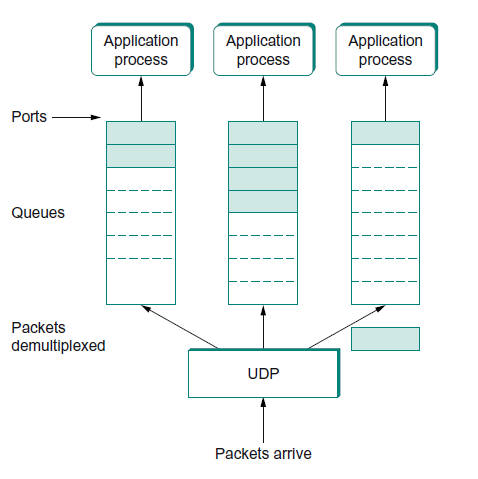
\includegraphics[width=0.5\textwidth
]{images/udp-message-queue.png}
	\caption[Cola de mensajes de UDP]{Cola de mensajes de UDP}
	\label{fig:udp-message-queue}
\end{figure}

Cuando llega un mensaje, el protocolo lo agrega al final de la cola. Si la cola está llena, el mensaje se descarta. No hay mecanismo de control de flujo en UDP para decirle al remitente que se ralentice. Cuando un proceso de aplicación desea recibir un mensaje, se elimina uno de la parte delantera de la cola. Si la cola está vacía, el proceso se bloquea hasta que haya un mensaje disponible.

Finalmente, aunque UDP no implementa el control de flujo o la entrega confiable / ordenada, también garantiza la corrección del mensaje mediante el uso de un cheksum. El mismo  toma como entrada el encabezado UDP, el contenido del cuerpo del mensaje y algo llamado \textbf{pseudoencabezado}. El pseudoencabezado consiste en tres campos del encabezado IP: número de protocolo, dirección IP de origen y dirección IP de destino, más el campo de longitud UDP. La motivación detrás de tener el pseudoencabezado es verificar que este mensaje se haya entregado entre los dos puntos finales correctos.

\subsection{Transmission Control Protocol (TCP)}
TCP garantiza la entrega confiable y en orden de un flujo de bytes. Es un protocolo full-duplex, lo que significa que cada conexión TCP admite dos flujos de bytes simulteanos en dirección opuesta. También incluye un mecanismo de control de flujo para cada uno de ellos, lo que permite al receptor limitar la cantidad de datos que el remitente puede transmitir en un momento dado. La idea de este mecanismo es limitar la velocidad a la que TCP envía datos, no por el bien de evitar que el remitente sobrecargue al receptor, sino para evitar que el remitente sobrecargue la red. Finalmente, al igual que UDP, TCP admite un mecanismo de demultiplexación que permite que varios programas de aplicación en cualquier host dado mantengan una conversación simultánea con sus pares. 

\subsubsection{Sliding Window en TCP}
TCP usa el algoritmo de ventana deslizante para asegurar la entrega confiable de los mensajes. Aunque este es el mismo algoritmo básico que vimos en la Sección \ref{sec:ventana-deslizante}, debido a que TCP se ejecuta a través de Internet en lugar de una conexión punto a punto, hay muchas diferencias importantes:
\begin{itemize}
  \item TCP admite conexiones lógicas entre procesos que se ejecutan entre dos computadoras cualquieras conectadas al Internet por lo que necesita una fase explícita de establecimiento de conexión durante la cual ambos nodos acurdan intercambiar información entre sí. Esto genera un estado compartido entre ellos que se usa para comenzar el algoritmo de ventana deslizante y que debe ser liberado cuando la conexión se cierra por lo que TCP también tiene una fase explícita de desmontaje de la conexión.
  \item Mientras que un solo enlace físico que siempre conecta las mismas dos computadoras tiene un tiempo de Round-Trip Time (RTT), las conexiones TCP probablemente tendrán tiempos de ida y vuelta diferentes dependiendo de la distancia entre ellas, la carga de la red, etc. Las variaciones en el RTT incluso son posibles durante una sola conexión TCP que dura solo unos minutos. Osea que el algoritmo de ventana deslizante debe tener un mecanismo retransmisiones con tiempos de espera adaptativos.
  \item Los paquetes pueden reordenarse a medida que cruzan el Internet. Los paquetes que están ligeramente desordenados no causan un problema ya que el algoritmo de ventana deslizante puede reordenar los paquetes correctamente usando el número de secuencia. El verdadero problema es cuán desordenados pueden estar los paquetes o, dicho de otra manera, cuán tarde puede llegar un paquete a su destino. En el peor de los casos, un paquete puede retrasarse en Internet hasta que expire el campo de tiempo de vida (TTL) de IP, momento en el cual el paquete se descarta (y, por lo tanto, no hay peligro de que llegue tarde). Sabiendo que IP descarta los paquetes después de que expire su TTL, TCP asume que cada paquete tiene un tiempo de vida máximo. El tiempo de vida exacto, conocido como tiempo de vida máximo del segmento (Maximum Segment Life - MSL), es una opción de ingeniería. La implicación es significativa: TCP tiene que estar preparado para que los paquetes muy antiguos aparezcan repentinamente en el receptor, lo que podría confundir el algoritmo de ventana deslizante.
  \item Casi cualquier tipo de computadora puede estar conectada a Internet, lo que hace que la cantidad de recursos dedicados a cualquier conexión TCP sea muy variable, especialmente considerando que cualquier host puede potencialmente admitir cientos de conexiones TCP al mismo tiempo. Esto significa que TCP debe incluir un mecanismo que cada lado usa para "aprender" qué recursos (por ejemplo, cuánto espacio de búfer) el otro lado puede aplicar a la conexión. Este es el problema de control de flujo.
\end{itemize}

\subsubsection{Formato de los segmentos}
TCP es un protocolo orientado a bytes, lo que significa que el remitente escribe bytes en una conexión TCP y el receptor lee bytes de la conexión TCP. Aunque "flujo de bytes" describe el servicio que el protocolo ofrece a los procesos de aplicación, el mismo no transmite bytes individuales a través de Internet. En cambio, en el host de origen, almacena en un búfer suficientes bytes del proceso de envío para llenar un paquete de tamaño razonable y luego envía este paquete a su par en el host de destino. En el host de destino, TCP vacía el contenido del paquete en un búfer de recepción, y el proceso de recepción lee de este búfer a su gusto.

Los paquetes intercambiados entre pares TCP se llaman segmentos, ya que cada uno lleva un segmento del flujo de bytes. Cada segmento contiene el siguiente encabezado:

\begin{figure}[H]
	\centering
	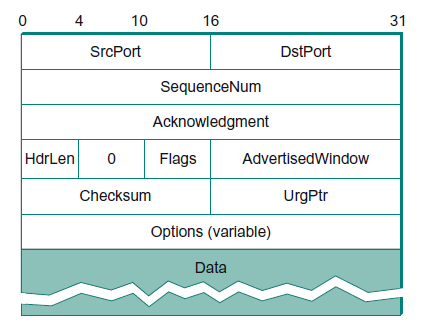
\includegraphics[width=0.5\textwidth
]{images/tcp-header.png}
	\caption[Encabezado de un paquete TCP]{Encabezado de un paquete TCP}
	\label{fig:tcp-header}
\end{figure}

\begin{itemize}
  \item \texttt{SrcPort} y \texttt{DstPort} identifican los puertos de origen y destino, respectivamente, al igual que en UDP. Estos dos campos, más las direcciones IP de origen y destino, se combinan para identificar de manera única cada conexión TCP. Es decir, la clave de demultiplexación de TCP está dada por la tupla de 4 elementos \texttt{SrcPort}, \texttt{SrcIPAddr}, \texttt{DstPort}, \texttt{DstIPAddr}.
  \item \texttt{Acknowledgment}, \texttt{SequenceNum} y \texttt{AdvertisedWindow} están involucrados en el algoritmo de ventana deslizante de TCP.
  \item \texttt{Flags} es un campo de 6 bits que se utiliza para transmitir información de control. Incluye los siguientes bits:
  \begin{itemize}
    \item \texttt{ACK} se establece cada vez que el campo \texttt{Acknowledgment} es válido, lo que implica que el receptor debe prestar atención a él. 
    \item\texttt{URG} significa que este segmento contiene datos urgentes. Cuando se establece este indicador, el segemento contiene datos urgentes desde el byte 0 hasta el byte \texttt{UrgPtr} 
    \item\texttt{PUSH} significa que el remitente invocó la operación de empuje, esto indica que el receptor debe poder leer la información contenida en el segmento apenas llegue.
    \item \texttt{RESET} significa que el receptor se ha confundido, por ejemplo, porque recibió un segmento que no esperaba recibir, por lo que desea abortar la conexión.
  \end{itemize}
  \item \texttt{Checksum} se usa exactamente de la misma manera que para UDP: se calcula sobre el encabezado TCP, los datos TCP y el pseudoencabezado, que está compuesto por los campos de dirección de origen, dirección de destino y longitud del encabezado IP. El checksum es obligatorio para TCP tanto en IPv4 como en IPv6. 
  \item \texttt{HdrLen} indica la longitud del encabezado TCP en palabras de 32 bits. Este campo también se conoce como el campo \texttt{Offset}, ya que mide el desplazamiento desde el inicio del paquete hasta el inicio de los datos.
\end{itemize}

\subsubsection{Establecimiento de una conexión TCP}
Una conexión TCP comienza con un cliente (caller) haciendo una apertura activa a un servidor (callee). Suponiendo que el servidor hubiera hecho una apertura pasiva anteriormente, los dos lados se involucran en un intercambio de mensajes para establecer la conexión. Solo después de que finalice esta fase, los dos lados pueden comenzar a enviar datos. De manera similar, tan pronto como un participante haya terminado de enviar datos, cierra una dirección de la conexión, lo que hace que TCP inicie una ronda de mensajes de terminación de conexión.

\subsubsection*{3-Way Handshake}
\begin{figure}[H]
	\centering
	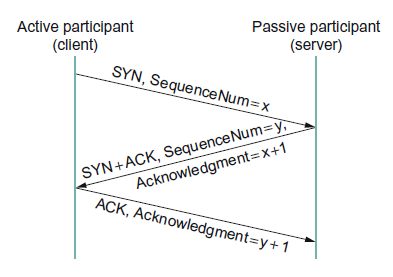
\includegraphics[width=0.5\textwidth
]{images/three-way-handshake.png}
	\caption[Intercambio de mensajes para 3-Way Handshake]{Intercambio de mensajes para 3-Way Handshake}
	\label{fig:three-way-handshake}
\end{figure}
El algoritmo utilizado por TCP para establecer y terminar una conexión se llama handshake de tres vías (Three Way Handshake).

Dos computadoras que quieran inicializar una conexión, deben acordar los números de secuencia de inicio que las dos partes planean usar para sus respectivos flujos de bytes. Primero, el cliente (el participante activo) envía un segmento al servidor (el participante pasivo) indicando el número de secuencia inicial que planea usar (\texttt{FLAG = SYN, SequenceNum = x}). El servidor responde con un solo segmento que reconoce el número de secuencia del cliente (\texttt{FLAG = ACK, Ack = x + 1}) y establece su propio número de secuencia de inicio (\texttt{Flags = SYN + ACK, SequenceNum = y}). Finalmente, el cliente responde con un tercer segmento que reconoce el número de secuencia del servidor (\texttt{Flags = ACK, Ack = y + 1}). La razón por la cual cada lado reconoce un número de secuencia que es uno más grande que el enviado es que el campo de reconocimiento realmente identifica el "siguiente número de secuencia esperado", reconociendo implícitamente todos los números de secuencia anteriores. Aunque no se muestra en esta línea de tiempo, se programa un temporizador para cada uno de los dos primeros segmentos, y si no se recibe la respuesta esperada, el segmento se retransmite.

\subsection*{Diagrama de transición de estados de TCP}
Todas las conexiones comienzan en el estado CLOSED. A medida que la conexión avanza, la conexión se mueve de un estado a otro de acuerdo con los arcos. Cada arco está etiquetado con una etiqueta de la forma evento / acción.

\subsubsection*{3-Way Handshake}
\begin{figure}[H]
	\centering
	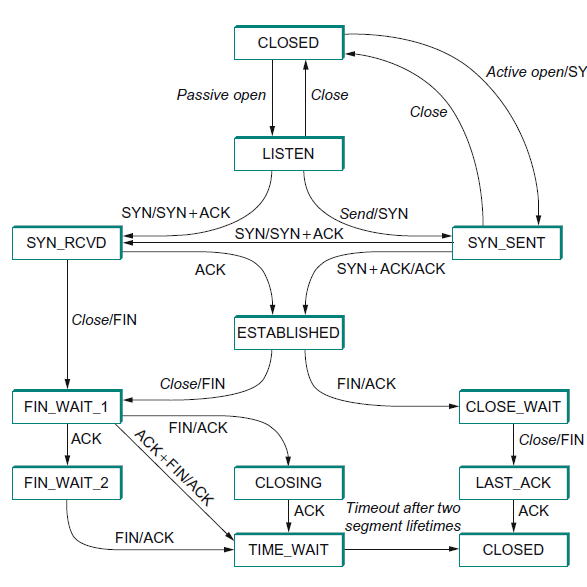
\includegraphics[width=0.5\textwidth
]{images/tcp-state-transitions.png}
	\caption[Transiciones de estado TCP]{Transiciones de estado TCP}
	\label{fig:tcp-state-transitions}
\end{figure}


\newpage

% Traducir del ingles
All
connections start in the CLOSED state. As the connection progresses, the
connection moves from state to state according to the arcs. Each arc is
labeled with a tag of the form event/action.
% Al español:
Todas las conexiones comienzan en el estado CLOSED. A medida que la conexión avanza, la conexión se mueve de un estado a otro de acuerdo con los arcos. Cada arco está etiquetado con una etiqueta de la forma evento / acción.